\begin{Pro}
    Para el siguiente automata, finito no determinista, construye el automata finito determinista equivalente.
\end{Pro}

\begin{proof}
    \begin{enumerate}
        \item Primero, identificamos los estados iniciales: 
        \begin{align*}
            S_0 &= \{q_0\} \cup \{r: q \in S_0 \land S(q,\epsilon)\} && \text{No hay epsilon transiciones}\\ 
            S_0 &= \{q_0\}
        \end{align*}
        \item Ahora, construimos la función de transición para el autómata determinista. Para cada estado en $S_0$, 
        determinamos las transiciones para cada símbolo de entrada.
        \begin{align*}
            \delta(S_0,a) &= \{q_1\}\ cup \epsilon-closure(\{q_1\}) \\ 
           &= \{q_1\} = S_1 \\
            \delta(S_0,b) &= \emptyset \\ 
            \delta(S_1,a) &= \{q_2\} \cup \epsilon-closure(\{q_2\}) \\
            &= \{q_2\} = S_2 \\
            \delta(S_1,b) &= \{q_0,q_2\} \cup \epsilon-closure(\{q_0,q_2\}) \\
            &= \{q_0,q_2\} = S_3 \\
            \delta(S_2,a) &= \{q_3\} \cup \epsilon-closure(\{q_3\}) \\
            &= \{q_3,q_0\} = S_4 \\
            \delta(S_2,b) &= \emptyset \\ 
            \delta(S_3,a) &= \{q_1,q_3\} \cup \epsilon-closure(\{q_1,q_2,q_3\}) \\
            &= \{q_0,q_1,q_3\} = S_5 \\
            \delta(S_3,b) &= \emptyset \\ 
            \delta(S_4,a) &= \{q_1,q_2\} \cup \epsilon-closure(\{q_1,q_2\}) \\
            &= \{q_1,q_2\} = S_6 \\
            \delta(S_4,b) &= \emptyset \\ 
            \delta(S_5,a) &= \{q_1,q_2\} \cup \epsilon-closure(\{q_1,q_2\}) \\
            &= \{q_1,q_2\} = S_6 \\
            \delta(S_5,b) &= \{q_0,q_2\} \cup \epsilon-closure(\{q_0,q_2\}) \\
            &= \{q_0,q_2\} = S_3 \\
            \delta(S_6,a) &= \{q_2,q_3\} \cup \epsilon-closure(\{q_2,q_3\}) \\
            &= \{q_0,q_2,q_3\} = S_7 \\
            \delta(S_6,b) &= \{q_0,q_2\} \cup \epsilon-closure(\{q_0,q_2\}) \\
            &= \{q_0,q_2\} = S_3 \\
            \delta(S_7,a) &= \{q_1,q_2,q_3\} \cup \epsilon-closure(\{q_1,q_2,q_3\}) \\
            &= \{q_0,q_1,q_2,q_3\} = S_8 \\
            \delta(S_7,b) &= \emptyset \\ 
            \delta(S_8,a) &= \{q_1,q_2,q_3\} \cup \epsilon-closure(\{q_1,q_2,q_3\}) \\
            &= \{q_0,q_1,q_2,q_3\} = S_8 \\
            \delta(S_8,b) &= \{q_0,q_2\} \cup \epsilon-closure(\{q_0,q_2\}) \\
            &= \{q_0,q_2\} = S_3   
        \end{align*}

        Como no tenemos nuevos estados terminamos. Ahora construimos los estados Finales
        \begin{align*}
            F &= \{S_0,S_3,S_4,S_7,S_8\} \\
        \end{align*}
    \end{enumerate}
    \begin{figure}[h!]
            \centering
            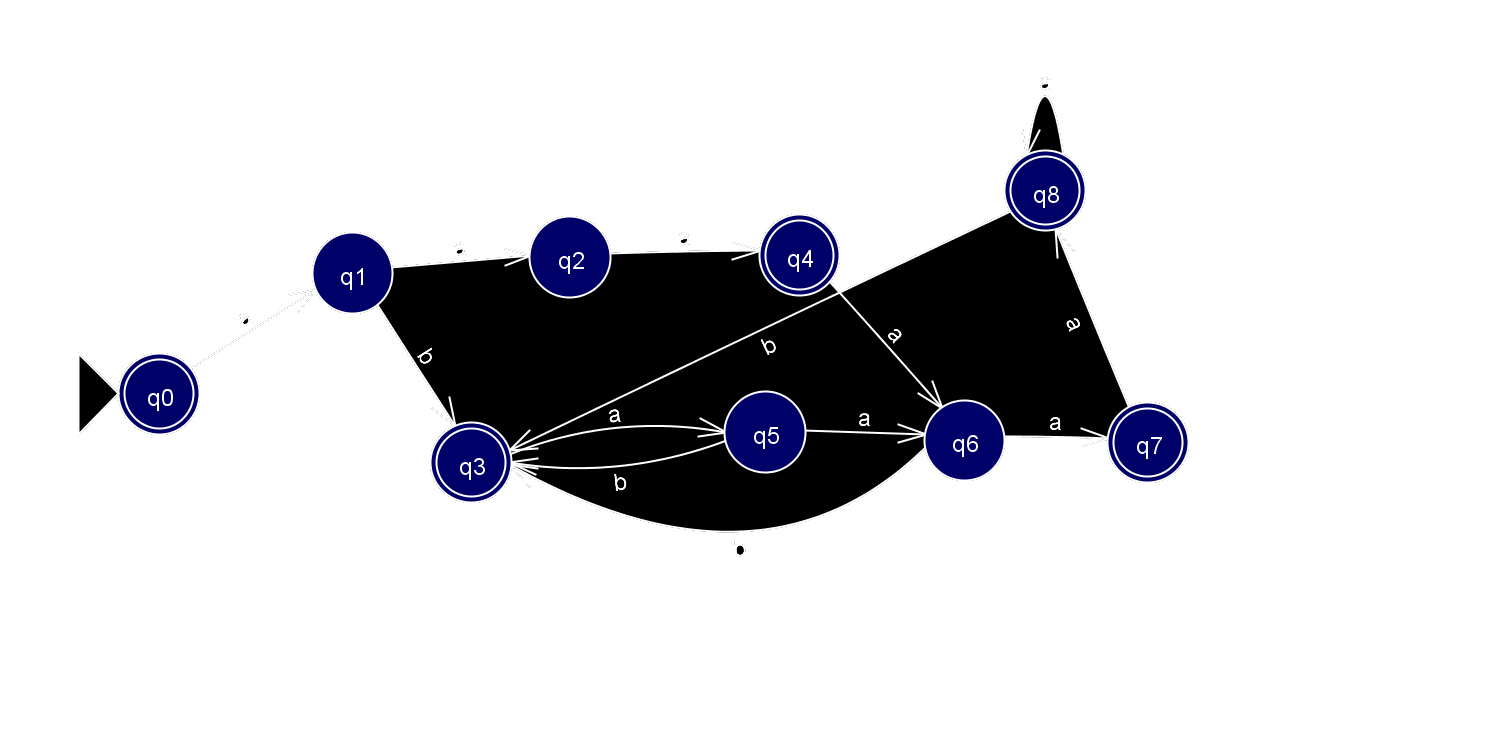
\includegraphics[width=\textwidth]{images/ejercicio5-bueno-dark.png}
            \caption{Automata Finito Determinista, ejercicio 5}
    \end{figure}
\end{proof}